\documentclass[12pt,a4paper,openany]{scrartcl}

\usepackage[sorting=none]{biblatex}
\addbibresource{biblio.bib}

\usepackage{mystyle}



\begin{document}
	%%% Maketitle metadata
\newcommand{\horrule}[1]{\rule{\linewidth}{#1}} 	% Horizontal rule


\title{
	%\vspace{-1in} 	
	\usefont{OT1}{bch}{b}{n}
	\normalfont \normalsize \textsc{DSSC - Advanced Programming} \\ [25pt]
	\horrule{0.5pt} \\[0.4cm]
	\huge AP Exam - Binary Search Tree \\
	\horrule{2pt} \\[0.5cm]
}
\author{
	\normalfont 								\normalsize
	Amadio Simone, Patrick Indri\\[-3pt]		\normalsize
    \selectlanguage{english}	
    \today
}
\date{}


	\maketitle
	
	
\section{Introduction}
	The aim of the project is to implement a binary search tree. Its performance should then be compared with \texttt{std::map}.\\
    The tree is templated on key and value type. A third template allows user defined class to be used as key, if a compare structure is provided. As default, the tree uses \texttt{std::less} to compare two keys.\\\\
    The code is organized in two folders: \texttt{include/}, which contains a header file, and \texttt{src/} which contains the implementation of the binary search tree and the \texttt{makefile}. The latter should be used to generate the executables to test and benchmark the implemented class. Please follow the instructions on the provided \texttt{README.md}.\\
    \texttt{test.cc} is used to test the functionalities and features of our class, using \texttt{std::cout} to show what method is being called and verify its validity, verifying error handling as well. Furthermore, we tested the correct behaviour of our \texttt{BSTree} with user defined classes such as \texttt{CustomKey} and \texttt{CustomKey\_Explicit}.
	
\section{Classes}
	\begin{itemize}
	    \item\texttt{BSTNode}: binary search tree node. Located on a different namespace with respect to the tree, this class implements the idea of a generic node in a binary search tree. It is implemented in a different namespace so that it is not exposed to the user, who cannot in any way access or modify by chance this class and its methods.Unlike the tree, the node is not templated on the compare function: this is another reason not to nest it in the BSTree class.
	    
	    Every node is defined by its members: a content, which is an \texttt{std::pair} of templated key and value, two unique pointers to children nodes (namely "left" and "right") and one "parent" raw pointer. The key is implemented as a \texttt{const}, since it should not be modified in order to preserve the ordering of the tree and not corrupt it.
	    
	    \item \texttt{BSTree}: binary search tree. It is completely identified by its members: a unique pointer to \texttt{BSTNode} which represents the root of the tree, to which all of the other nodes are appended. We decided also to add the size of the tree as member, considering it can be useful.
	    
	    \item \texttt{Iterator}. Its only member is a pointer to \texttt{BSTNode}. Through the overloading of the operator ++, allows cycling through the nodes of the tree in key order. If deferenced, returns the content of the node it's pointing to.
	    
	    \item \texttt{ConstIterator}. Similar to the iterator, but can be used inside \texttt{const} functions.
	    
	    \item \texttt{Error}. Auxiliary structure used to throw and catch errors at run time.
	    
	    \item \texttt{CustomKey} and \texttt{CustomKey\_explicit}. Auxiliary structures used to test tree behaviour on custom keys and with custom ordering.
	\end{itemize}
	

\section{Main methods}

\begin{itemize}
    \item \texttt{position\_of()}. Auxiliary private function used both by the \texttt{insert()} and the \texttt{find()} methods. It takes as argument a key: if the key is found within the tree, it returns an iterator pointing to the node in which it's contained. If the key was not already present in the tree, it returns an iterator pointing to the to-be parent node.
    \item \texttt{find()}. It takes a key as argument and returns an iterator pointing to the node the key is contained in. If the key's not found, it returns \texttt{cend()}.
    \item \texttt{insert()}. Public method: it takes a key and a value and inserts a new node in the tree. Key and value can be passed both separately or contained within an \texttt{std::pair}. If the key chosen is already present, it does not override the previous content. The method returns a boolean which is \texttt{True} if a new node was appended, \texttt{False} if the key was already present.
    \item \texttt{print()}. It prints the content of all the elements of the trees using the overload of the operator \texttt{<<}. The content is printed according to key ordering.
    \item \texttt{balance()}. Balance the tree. It creates a vine (linearized version of the tree, similar to a linked list) ordered by key. After inserting the median key, it recursively bisects the vine, inserting the median element of each bisection.
    \item \texttt{operator[]}. It takes a key as argument and returns the corresponding value. It's implemented in two different versions: \texttt{const} and non-\texttt{const}.
    
    In the \texttt{const} version, searching for a non-existent key throws an exception, since the tree is not supposed to be modified.
    
    In the non-\texttt{const} version, searching for a non-existent key provokes a new node to be created, containing the given key and the default value for the value type. This new insertion is advised to the user through a printed message.
    
    \item \texttt{operator==}. Returns \texttt{True} if the sizes of the trees and the content of every node are the same. It does not check the structure of the tree (insert-order dependent). If the same structure is needed, balancing the trees whose \texttt{==} returned \texttt{True} will achieve the aim.
\end{itemize}


	\noindent Copy and move semantics for the \texttt{BSTree} were implemented as well. For more details on the implementation of the classes and their methods, please refer to the Doxygen documentation, provided in the \texttt{doc} folder.
	
\section{Custom key ordering}
	With custom classes as key, an ordering must be provided by the user. Testing our code we verified that an user can provide such ordering in two different ways:
		
	\begin{itemize}
		\item Define a functor to be passed as the third template in defining \texttt{BSTree}.
		\item Overload the operator less than "<" with respect to the key class. Our code uses as default std::less, which, unless specified, exploit the "<" operator. In this case, there is no need to pass anything as a third template.
	\end{itemize}
	
	\noindent The user should be aware that if two keys are not greater (\texttt{<}) nor  smaller (\texttt{>}) with respect to each other, in this class they will be considered as equal.
	
	\section{Benchmark}
	\texttt{benchmark.cc} provides the code we used to benchmark our \texttt{BSTree}.\\
	We tested the effectiveness of our \texttt{find()} function and compared it with \texttt{std::map}. We tested both on a random unbalanced tree and on its balanced conversion. We chose double variables as keys. First, we populate a \texttt{std::vector} with an increasing sequence of doubles, in interval $[0,1]$. Then, we randomly shuffle the vector: this procedure generates a random vector of doubles with no repetitions. We finally insert each element in a \texttt{BSTree}. This procedure should result in randomly generated trees.\\
	
	\noindent We used the \texttt{find()} function to search through all the keys in the data structures and sum up the time taken. For each dimension we took the average performance over 5 random trees, in order to minimise fluctuations. The results are shown in the following plots.
	
    \begin{figure}[H]
        \centering
        \captionsetup{format=plain}
        \caption{On $y$ axes, $log(time)$. Times in $\mu s$. Mean of 5 runs for each number of nodes.}
        \label{fig:O0}
        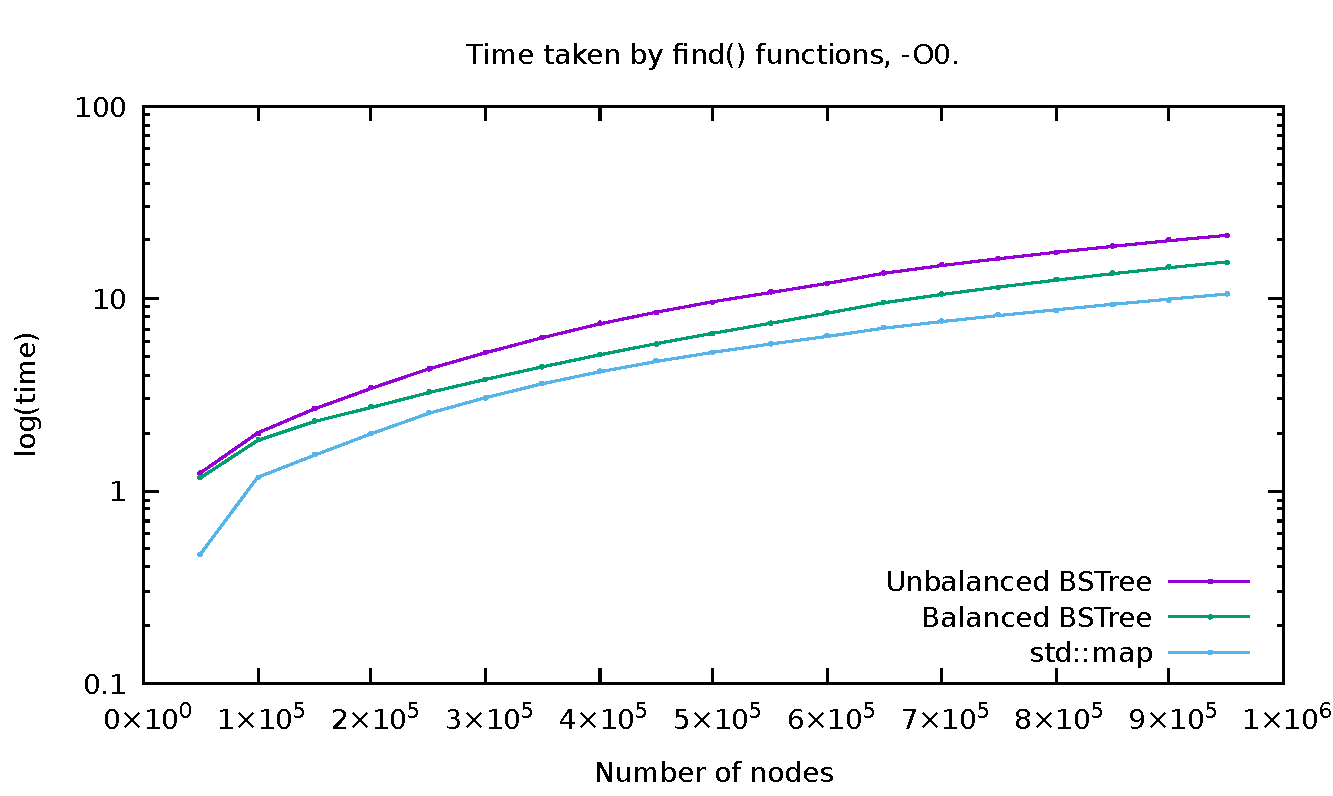
\includegraphics[width=0.85\textwidth]{img/plotO0.pdf}
    \end{figure}
    
    \begin{figure}[H]
        \centering
        \captionsetup{format=plain}
        \caption{On $y$ axes, $log(time)$. Times in $\mu s$. Mean of 5 runs for each number of nodes.}
        \label{fig:O3}
        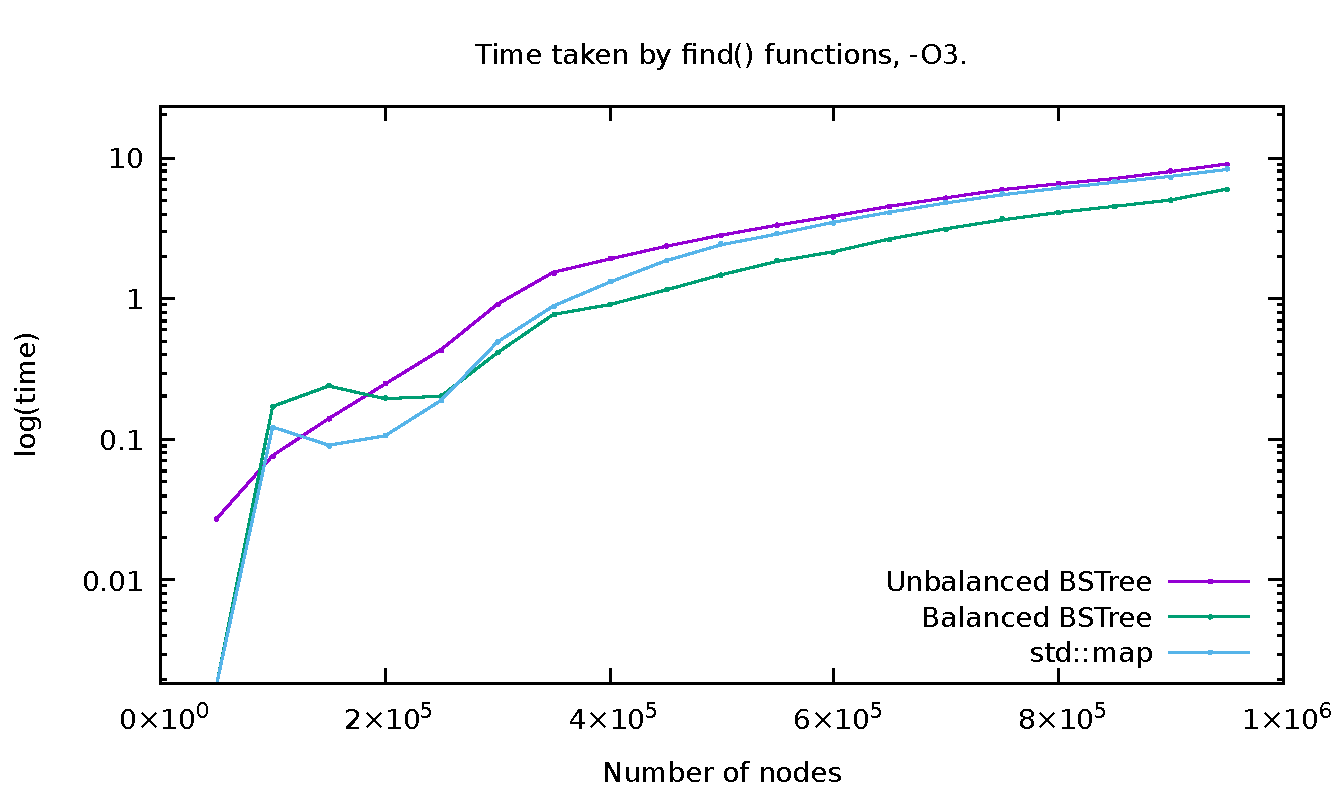
\includegraphics[width=0.85\textwidth]{img/plotO3.pdf}
    \end{figure}
    
    	
	We ran our test both on \texttt{-O0} and \texttt{-O3} optimisation levels. It seems that using \texttt{-O0} the \texttt{std::map} is faster than our tree, probably because it's implemented in an optimised fashion. Using \texttt{-O3} on the other hand, our code runs faster, probably because our simpler code can be more easily optimised.
	
	We expect the balanced tree and \texttt{std::map} to have a $log(N)$ complexity for the find function, resulting in a linear behaviour in the plots. We can see that for a sufficient number of nodes, this hypothesis seems to hold. 
	
\end{document}
